\documentclass[12pt,a4paper,oneside]{book}
\usepackage[a4paper,%
            left=35mm,right=20mm,top=20mm,bottom=20mm]{geometry}
\usepackage{titlesec} 
\usepackage{fancyhdr}
\usepackage[utf8]{inputenc} 
\usepackage{graphicx}
\usepackage{booktabs} % for much better looking tables
\usepackage{array} % for better arrays (eg matrices) in maths
\usepackage{paralist} % very flexible & customisable lists (eg. enumerate/itemize, etc.)
\usepackage{verbatim} % adds environment for commenting out blocks of text & for better verbatim
\usepackage{subfig} % make it possible to include more than one captioned figure/table in a single 
\usepackage[toc,page]{appendix}
\usepackage{pdfpages}
\usepackage{listings}
\usepackage{color}
\usepackage{graphicx}
\usepackage{subfig}
\usepackage{setspace}
\onehalfspacing
\usepackage{helvet}
\usepackage{mathtools}

%Hyperlinks set to no colours/black
\usepackage{hyperref}
\hypersetup{
    colorlinks=false,
    linkcolor=black,
    filecolor=black,      
    urlcolor=black,
}

\renewcommand{\familydefault}{\sfdefault}

\definecolor{dkgreen}{rgb}{0,0.6,0}

%header and footer settings
\pagestyle{fancyplain}
\fancyhf{}
\renewcommand{\headrulewidth}{0.5pt}
\renewcommand{\footrulewidth}{0.5pt}
\setlength{\headheight}{15pt}
\fancyhead[L]{Adam Blance - 40161070}
\fancyhead[R]{ SOC10101 Honours Project}
\fancyfoot[L]{}
\fancyfoot[C]{\thepage}



%set better section layout
\makeatletter
\renewcommand\subsection{\@startsection {subsection}{1}{2mm} % name, level, indent
                               {3pt plus 2pt minus 1pt} % before skip
                               {3pt plus 0pt} % after skip
                               {\normalfont\bfseries}}
\makeatother
\makeatletter
\renewcommand\section{\@startsection {section}{1}{0mm} % name, level, indent
                               {4pt plus 2pt minus 1pt} % before skip
                               {4pt plus 0pt} % after skip
                               {\bfseries}}
\makeatother


%this starts the document
\begin{document}

\frontmatter

%you can import other documents into your main one, these layout the Title and Declarations on its own page.
%you might need to change these to \ if your on Microsoft Windows.
\newcommand{\HRule}{\rule{\linewidth}{0.5mm}}

\begin{titlepage}
	\begin{center}

	\HRule \\[0.4cm]
    	{\Large \bfseries Evaluation of Procedaully Generatated Escort Mission Maps\par}
	\vspace{0.2cm}
	\HRule \\[1.5cm]

	
    	\vspace{3cm}
	\begin{minipage}{0.4\textwidth}
	\begin{center} \large
        \emph{}\\
        	Adam Blance - 40161070
				
   	 \end{center}
    	\end{minipage}
	
	\vspace{2cm}
    	\begin{minipage}{1\textwidth}
    	\begin{center} \large
        
		Submitted in partial fulfilment of \\
		the requirements of Edinburgh Napier University \\
		for the Degree of \\
        	BSc (Hons) Games Development
    	\end{center}
    	\end{minipage}

    	\vfill

    	% Bottom of the page
	\begin{minipage}{1\textwidth}
    	\begin{center} \large
		School of Computing
    	\end{center}
    	\end{minipage}
	
	\vspace{1cm}
    	{\large \today}


	\end{center}
\end{titlepage}
%{\large Submitted in partial fulfilment of the requirements of Edinburgh Napier University for the Degree of }

\section*{Authorship Declaration}
\vspace{0.5cm}
\begin{flushleft}
I, Adam Blance, confirm that this dissertation and the work presented in it are my own achievement.\newline

Where I have consulted the published work of others this is always clearly attributed;\newline

Where I have quoted from the work of others the source is always given. With the exception of such quotations this dissertation is entirely my own work;\newline

I have acknowledged all main sources of help; \newline

If my research follows on from previous work or is part of a larger collaborative research project I have made clear exactly what was done by others and what I have contributed myself;\newline

I have read and understand the penalties associated with Academic Misconduct.\newline

I also confirm that I have obtained informed consent from all people I have involved in the work in this dissertation following the School's ethical guidelines.\newline
\end{flushleft}

\begin{flushleft} \large
\emph{Signed:} \\
\end{flushleft}

\vspace{.5cm}

\begin{flushleft} \large
\emph{Date:} \\
\end{flushleft}

\vspace{.5cm}

\begin{flushleft} \large
\emph{Matriculation no: }  \\
\end{flushleft}
\pagebreak

\section*{Data Protection Declaration}
\vspace{0.5cm}
\begin{flushleft}
Under the 1998 Data Protection Act, The University cannot disclose your grade to an unauthorised person. However, other students benefit from studying dissertations that have their grades attached. \newline

\vspace{0.5cm}

Please sign your name below one of the options below to state your preference.\newline
\vspace{0.5cm}

The University may make this dissertation, with indicative grade, available to others.\newline
\vspace{3cm}


The University may make this dissertation available to others, but the grade may not be disclosed.\newline
\vspace{3cm}


The University may not make this dissertation available to others.\newline
\end{flushleft}


\pagebreak

\section*{Abstract}
Being able to evaluate certain types of maps can be a very useful tool for game developers of first person shooters. These games can be extremely popular.With the one of largest still boasting a player base of over 30 million a year after the game was released \cite{OverwatchPopularity}. This means that company who could quickly evaluate and release their games could beat out competitors, with the most successful of these likely securing a higher profit margin.
\vspace{5mm} 
\newline
 This dissertation will document the research, implementation and evaluation of an attempt to successfully automate the evaluation process of the release co-operative first person shooter maps and an attempt to procedurally generate these maps was made. We aim to identify what makes a good map and what factors effect the success of these maps.
 \vspace{5mm} 
 \newline
 We look at a variety of games that are currently on the market and have a large player bases along with the maps that are considered the most popular within them. We investigate the similar projects like this and identify the several techniques that maybe suitable for generating a map that can be used to successfully pass the algorithm.
  \vspace{5mm} 
 \newline
 A detailed analysis on these techniques is provided. Also included is the outlining of the process of creating the noise that was generated adhering to the evaluation algorithm and the aspects that are used including Dijkstra's algorithm and binomial distribution. We also discuss the creation of the survey that will be used to test the successfulness of the algorithm and discuss the metrics which will be recorded. 
  \vspace{5mm} 
 \newline 
 The implementation provides a detailed description of the creation process of the evaluation algorithm. A description is provided on the creation of the procedural generated map that was also created. The challenges that were encountered during these tasks are also highlighted.
  \vspace{5mm} 
 \newline 
 Analysing the results we were able to draw a number of conclusions;--------------------------------------------------AAAAAA
\tableofcontents 

\listoftables

\listoffigures

\newpage
\section*{Acknowledgements}
I would like to thank my supervisor, Dr Kevin Chalmers, for all his constant support, thorough out my time in university and I am incredibly grateful for all the times he has listened to and helped with all my concerns and problems.  
 \vspace{5mm} 
\newline 
I would also like to thank my second marker, Dr Gregory Leplatre for his  encouragement,support, and helpful advice that he has given during my time in university.
 \vspace{5mm} 
\newline 
I am also greatly  thankful for all my course mates and my family who have helped me out so much during this year and I greatly valued all the time we have spent together. 
 \vspace{5mm} 
\newline 
Finally I would like to thank the School of Computing for giving me the facilities needed to create this dissertation and give me the knowledge that will help me for the rest of my life.
\newpage

\mainmatter

%INTRO
\chapter{Introduction}
From the beginning of the project the objective has been to develop a mathematical equation to evaluate escort mission maps. Then to procedurally generate maps that can successfully follow the evaluation technique created. The dissertation produced underneath documents the work that was involved in achieving this.
\section{Motivation}
With video games being one of the largest markets in the world right now, gaming companies must be developing and releasing their games as quickly as possible. If there is any conceivable way for them speed up releasing their games, they should take these approaches.
\vspace{5mm} 
\newline  
One of the biggest genres of games currently is team based shooters. With one of the larger games in the genre being Overwatch with currently over 35 million players worldwide. \href{https://twitter.com/PlayOverwatch/status/919925924769906688}. This genre of game has a very different development cycle to other games relying on continual updates adding new maps and characters to keep players interested and continually playing. To release new maps and characters on a regular basis can be difficult especially if the game has a large competitive scene because the new feature \vspace{5mm} must be fully tested before released.
\newline  
With testing new features in games becoming the most time consuming part of the development cycle, companies must look into other ways to streamline the testing of games. In this project one of the possible ways to decrease the time taken to test maps is explored. If companies can use a mathematical formula to test the fairness of maps, rather than the more conventional user based testing which can take up to several weeks, would allow for companies to produce more content in a quicker time frame, generating a greater profit and allowing for better content to be produced in the future. 
\section{Aims and Objectives}
There are two main aims of the project, the first is to create, implement and evaluate an algorithm that assesses escort mission maps once this has been complete, the next aim is to plan and develop a piece of software that can successfully follow the algorithm produced. The objectives below have been selected in order to accomplish these aims.
\begin{itemize}
	\item Research relevant topics and papers.
	\item Create or use an existing framework that can be used to develop the map.
	\item Design an algorithm taking into account size, path of the payload and fairness. 
	\item Develop a programme that can procedurally generate escort mission maps.	
\end{itemize}
\section{Scope}
\subsection{Deliverable}
The items to be delivered from this project are: An algorithm that can evaluate any escort mission map and inform the user of the strengths and weakness of the map; A C++ program that can procedurally generate maps that can be tested by the algorithm; the results and analysis of the surveys that examine the credibility of the evaluation algorithm.  
\subsection{Boundaries and Constraints}
When testing a map there are a large amount variables to be evaluated, as time is one of the limiting factors in this project, it was decided that 3 major factors would be tested. They are:
\begin{itemize}
	\item The size of the map.
	\item The quality of the object that will be escorted (payload) path.
	\item The overall balance\textbackslash fairness of the map 	
\end{itemize}
\section{Chapter Outlines}
\begin{itemize}
	\item Background - Discusses the research made into the topic.
	\item Methodology – States the methods used throughout the implementation process.
	\item Implementation - Details specific techniques and choices that were made during the Implementation phase.
	\item Results – Displays the results from the tests carried out.
	\item Conclusion – Summarises results that were collected , assess the successfulness of the data gathered and discusses future work.	
\end{itemize}

%BACKGROUND
\chapter{Background}
In this section, an investigation into escort mission maps and how to evaluate them is presented. Requirements and challenges are presented, and in particular video game maps are examined. Procedural generation one of the main factors of this project is also examined in depth. Finally path-finding and other evaluating techniques is presented, focusing on how to evaluate maps in video games. 
\vspace{5mm} 
\newline
\section{Co-operative First Person Shooters}
First Person Shooters are a large video game genre that have dominated the market for over 20 years with one of the first major titles being Quake in 1996 and other notable series including Call of Duty, Battlefield and Halo, with the objective of the game usually being to get the most eliminations. 
\vspace{5mm} 
\newline
A subsection of this genre is the co-operative first person shooter. This type of game heavily relies on teamwork, with games being won by holding onto an objective or pushing a payload. These games are enjoyable to a wide player base, usually offering a variety of play styles or different characters to use. This attracts a wide player base which translates to a large amount of revenue streams for the company that produced these games; including E-Sports, merchandises and potential Spin-off games. This include Blizzards co-op game Overwatch hitting peak viewer-ship with 441,000 viewers on its English stream during its first day \cite{LukeChristou}
\subsection{Escort Missions}
An escort mission is a game-mode in cooperative first person shooter such as Overwatch and Loadout. In this mode there are two teams, the attacking and the defending team. The two teams have different aims in order to win. The attacking team attempts to escort the payload across the map to an objective while the defending team tries to stop them. It is difficult to pin down the first game to have escort missions. One of the more notable was in 2007 with Team Fortress 2. While it was not originally included in the game it was added in the first free update. It is important to note that the original Team Fortress had a game mode called Escort but this has many differences with its sequel, such as the payload being a controllable player and there being three teams. Other games that use this game mode include Global Agenda and Wolfenstein: Enemy Territory.    
\vspace{5mm} 
\newline
\section{Maps}
In video games, maps are the term used to describe the area that the player can move around in. Different games will have different types of maps depending on how the developer wants the player to play the game. For instance an RPG like Skyrim or The Witcher will usually have a large map for the player to explore the world and find their own path, while other faster paced first person shooters like the Call of Duty franchise might rely on a more linear map to construct the most enjoyable experience for their players. It is very important for a programmer to constantly be planning and evaluating the map they are creating as this will directly affect how enjoyable the game they created is.
\vspace{5mm} 
\newline
\section{Escort Mission Maps}
Escort mission maps are the play areas that escort missions are performed in. Between each game these maps can vary greatly so for this project, the definition of an escort mission map must be stated. The maps must have an attacking and defending spawn area. This is the place where the teams start at the beginning of the match and will return too whenever they die. The map must also have an unobstructed route that runs between the spawns, which the payload will be moved through. This route will be generated using path-finding algorithm which is discussed below.
\vspace{5mm} 
\newline 
\section{Procedural Generation in Video Games}
Typically when a game is being made their is a time constraint as the company will not have the resources to spend a large period of time developing their game. Usually data will have to be created manually which can be very time consuming, however several short-cuts can be made.
\vspace{5mm} 
\newline
Procedural generation is a technique that can be used  to generate data algorithmically and can be used to greatly reduce the time taken for the creation of large systems within the game. This can lead to a less predictable game and can also reduce the memory size of the game. It has been used in several large title such as; an entire galaxy in No Man's Sky and was used in the weapon generation in the very popular Borderlands series.  
\subsection{Procedurally Generated Maps}
It is very common in gaming to use procedural generation, as it allows companies to take short-cuts when creating the game, and allows them to focus on more time consuming aspects of the game such as; graphics and game-play. Procedural generation has been used in many video games for a variety of things. This includes weapon generation in the Borderlands series and Spore which uses procedural generation to create animals and evolve them. However the most common use of procedural generation is to create the map. This has been used in many notable games including, Minecraft , No Man’s Sky and Dwarf Fortress. These create huge worlds for the player to roam around in and can allow the map to go on forever. Procedural generation will be used in the project on a much smaller scale then most games to generate the map but it will be used in conjunction with other techniques such as path-finding.  
\vspace{5mm} 
\newline
\section{Path-Finding}
Many games today have implemented an advanced artificial intelligence for a variety of reasons, an important aspect of this path-finding. This is used for a variety of reasons such as enemy’s movement and being used for troop movements in real time strategy games. Path-finding is way for a computer to calculate the shortest route between two points. It does this by searching a graph by starting at one vertex and evaluating the neighbouring nodes. The most common of the path-finding algorithms is Dijkstra's algorithm.	
\subsection{Dijkstra’s Algorithm}
Published by Edsger W. Dijkstra in 1959, Dijkstra’s algorithm is a way to calculate the shortest path between nodes on a graph. Solving the single-source shortest path problem. Nodes on a graph can represent either a 2-dimensional grid or points in a 3-D space. The most common example of a real life application of Dijkstra’s algorithm is being used in geographical maps to plot the fastest route between two cities, where each city is a node and the roads are associated with a weight. 
\vspace{2mm} 
\newline
\begin{figure}
	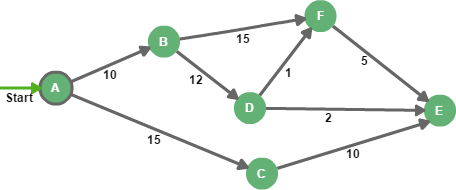
\includegraphics[width=\linewidth]{images/Dijsk.png}
	\caption{A weighted graph of connected nodes}
\end{figure}
The algorithm works by initially marking the distance from the starting point to every other vertex on the graph. All nodes are then set to unvisited and are stored  by priority within a queue. The next step would be to compare all unvisited neighbours and calculate the distance to travel between each node. For example, in figure 2.1 below if we are at the node A and wish to travel to node E, first we would look at the neighbouring nodes B and C. If the distance is less than the previous node than we add the current node to the path. Once all neighbouring nodes have been visited the current node is removed from the unvisited set and it will not be checked again. This process retreats until all nodes have been visited. At this time the graph will only contain the shortest paths from the source and a search can begin of the graph to find the shortest route to any node.
\subsection{A Star Path-finding (A*)}
The A* algorithm was first presented in 1968 by Peter E. Hart as an improvement on Nils Nilsson’s A1 algorithm. A1 was designed to be a heuristic approach to increase the speed of Dijkstra’s algorithm invented back in 1964. A* is a search based algorithm that attempts to calculate the most optimal route to a specified goal by travelling through a weighted graph. 
\vspace{5mm} 
\newline
The algorithm works by searching the nodes surrounding the current node using heuristic that estimate the distance from the end node.  A* contains two lists which are used to sort the nodes, open and closed. The open list contains all the nodes yet to be evaluated, while the closed list contains the nodes that have been assessed. Each node is given their own cost which is used to find the best path with the smaller cost the better. The score is calculated using the formula:
\[f(n) = g(n) + h(n)\]  
Where G is cost of travelling to the node and the h cost also known as the Heuristic cost is the cost to travel to the goal. This can be calculated in several ways and determines the efficiency and effectiveness of the algorithm. The F cost is the total cost of adding the two values together.
\vspace{5mm} 
\newline
The total cost is used by A* to guide the algorithm towards the goal. At each iteration of the algorithm the node with the lowest total cost is removed from the open list and its neighbours are evaluated. This involves searching the closed list to see if the neighbour has already been evaluated and checking if the node cannot be passed. If either of these cases are true then ignore the node, otherwise the node is checked to see if it exists in the open list, if it is not its F cost is calculated and the node is added to the open list. If the node already exists in the open list then its G cost is compared with the current lowest G cost, if the new G cost is lower than this is the better path. This process progresses until the goal has been evaluated and added to the open list or all nodes have been evaluated and the open list is empty, if this happens the goal cannot be reached from the start point.
\vspace{5mm} 
\newline
The two main methods for calculating the heuristic value are Euclidean distance and the Manhattan distance. Euclidean distance uses  Pythagorean Theorem to calculate the distance between the two points. This is the more popular heuristic as it is impossible to incorrectly calculate the value. This is because the shortest path between two points will always be a straight line. The Manhattan distance calculates the distance by discovering the sum of the differences between the two nodes.
\vspace{5mm} 
\newline
\section{Evaluations}
The process of evaluation can be done using several different techniques; Formative, Summative, Process and Impact. Formative evaluates the program during the development in order to make early improvements.A summative evaluation is conducted after the programme is released, this can be used to decide whether their should be extra content added or not. Process evaluation is used to determine if specific strategies used in the development cycle were useful and can be used to determine why the game has changed so much. The impact evaluation is a long term assessment to see how the game has affected the market over a long period of time. While the algorithm that is developed during this dissertation could be used for any one of these techniques it was decided that it would be used as a Formative evaluation as the algorithm could aim be most useful at this point because of its speed and real-time applications.  
\subsection{Evaluating Maps}  
 The process of evaluating maps can be very difficult. Each map must be tailored to enhance the player experience, while free-roam games aim to make the map as large  possible to encourage player exploration, other games have different priorities. This is especially the case in competitive shooters as the companies main aim to balance the game. This can be very hard as there are many aspects to creating a balanced game. A main part of this can include changing map objectives or reducing the size of the map. Each gaming company has their own private way of balancing these games but usually they will heavily rely on playing the map repeatedly, however this can lead to delayed release dates which can greatly affect the money they make of their game.
\vspace{5mm} 
\newline
\section{Related Work}
In the past couple of years the popularity of co-operative first person shooters has risen and more games have been using procedural generation. With popular titles such as Stardew Valley and No Man's Sky being released within the past year, however because of how competitive the video game market is these companies keep all their techniques and user data secret. The following documents will present some background on the techniques that are useful in this project.
\vspace{5mm} 
\newline
Stefan Greuter, Jeremy Parker, Nigel Stewart and Geoff Leach from Melbourne created a system that generated 'pseudo infinite' cities. The looked at creating geometrically varied buildings that's size depended on the buildings position. This was incredibly useful to compare as while this did not directly relate to the area that this dissertation was focusing on it could be applied to the building generation that was going to be used in the application \cite{StefanGreut}. 
\vspace{5mm} 
\newline
Another interesting paper that was on a similar topic was E. Galin's , A. Peytavie's,N. Maréchal's and E. Guérin's paper on procedural generation of roads \cite{Roads}. They looked into creating an automatic method of generating roads using a weighted anisotropic shortest path algorithm. They hoped to use this in simulations and using in the film industry. The main section of the paper outlines the discrete anisotropic path algorithm they created to generate tunnels and roads. They also discuss the main issues of the shortest path problem and why it is still a very relevant issue today.  They solve the shortest path problem using the A* algorithm that was described in section 2.0.5 however they created their own cost function that A* uses which they go on to describe in the next section. 
\vspace{5mm} 
\newline
Galin's cost function is a defined global function that uses several weighting factors that evaluate the influence of different effects of the terrain on the road. They defined this as:  
\begin{equation}
c(p,\dot{p}, \ddot{p}) = \displaystyle\sum_{i=0}^{i=n} \mu_i\circ\kappa_i(p,\dot{p}, \ddot{p})
\end{equation} 
This function while not highly relevant to the topic of this project did have a interesting concept that could be applied to the application. This was the value \(\mu_i\). This is the transfer function that allows the user to control the influence of the parameters being passed through the heuristic algorithm which could be modified to allow the computer to control the A* algorithm. 
\vspace{5mm} 
\newline
A very valuable paper to this project was Ricardo Lopes and Rafaels Bidarra's Adaptivity Challenges in Games and Simulations \cite{Fun}. This paper discusses the importance of adaptivity within games, while explaining that without adaptivity a company can alienate their player base and lose them to other games. While not the main focus of the article Lopes and Bidarra dedicate a section to game worlds. They reference many interesting investigations that researchers are currently conducting into procedural generating maps with a focus on giving more control to designers. Including the CityEngine which allows users to control the generation of a modern 3-D city.   ---------
%METHODologhy
\chapter{Methodology}
This chapter details the methods which will be used in the implementation stage. An overview will be provided of the techniques that were used and 
\section{Gradient Noise}
Gradient noise is a form of noise that is used to procedurally generate a texture 
\subsection{Perlin Noise}
Perlin Noise was created 
\section{Binomial Distribution }
\section{A* Modifications}
\section{Height Mapping}

%IMPLEMENTATION
\chapter{Implementation}
This section contains an in depth description of both the creation of the evaluation algorithm and the implementation of the procedurally generated co-operative first person shooter map. We will present the thematic choices that were made to optimize the successfulness of the map generation and the graphical choices such as height mapping that were made to easily visualize the map that was generated. To ensure the successfulness of both of the deliverables a survey was created that would allow the algorithm to be tested against users.
\vspace{5mm} 

\section{Programming Environment}
The applications were developed using Visual Studio 2017 Ultimate (Microsoft
2017) with the algorithm and application being written in C++. The graphics framework that was used was a combination of OpenGl and GLM \cite{OpenGL}. This allowed easy graphic manipulation which was important as it allowed more time to be spent on other aspects of the project.Through adding a header file that was imported from Github that already contained the Perlin noise algorithm within it, this helped with the exporting of image files that made it possible to easily view the terrain that had been generated. The survey was created using Microsoft Word to simplify the editing process for the users.  
\vspace{5mm} 
\newline
\section{Map Representation}

\section{Thematics}
\subsection{City}
\subsection{Desert}
\subsection{Village}
\subsection{Seaside}
%EVALUATION
\chapter{Evaluation}
Evaluation rubbish goes here

%CONCLUSION
\chapter{Conclusion}
Conclusion rubbish goes here

\newpage

\bibliographystyle{plain}
\bibliography{bibfile}

\newpage
\begin{appendices}
\section*{A Initial Project Overview Document}

\section*{B Week 9 Interim Report}

\section*{C Diary Sheets}

\section*{D Timeline}

\end{appendices}

\end{document}
